\documentclass[11pt, a4paper]{article}

\usepackage{graphicx}
\usepackage[english]{babel}
\usepackage[utf8x]{inputenc}
\usepackage{amsmath}
\usepackage{subfig}

\usepackage[a4paper,top=3cm,bottom=2cm,left=2cm,right=2cm,marginparwidth=1.75cm]{geometry}
\graphicspath{ {./images} }


\makeatletter
\renewcommand*\env@matrix[1][*\c@MaxMatrixCols c]{%
  \hskip -\arraycolsep
  \let\@ifnextchar\new@ifnextchar
  \array{#1}}
\makeatother

\begin{document}

\setcounter{section}{6}
\section{Lecture 7 (02/03/2020)}

\subsection{The concept of momentum and impulse}
Momentum (impuls in het Nederlands) was first formulated by Isaac Newton and is a way of measuring the amount of motion. The mathematical
description takes the following form:
\begin{equation}
  p = mv
\end{equation}
A force in turn is desribed as a change in momentum over time. Using calculus will give the following form:
\begin{equation}
  F = \frac{dp}{dt} = m\frac{dv}{dt} = ma
\end{equation}
Note that the equation $F = ma$ only holds in situation where the mass is constant. For almost all systems
we concern ourselfs with in dynamics this is true. However this is not always the case when for example
describing a fluid flow. In cases like these force needs to be described using an integral. This looks
like the following:
\begin{gather}
  \int_t F\,dt = \int_t ma\,dt = \int_t m\frac{dv}{dt}\,dt = \int_v m\,dv\\
  \int_t F\,dt = \Delta mv = \Sigma m_iv_{i,2} - \Sigma m_iv_{i,1}
\end{gather}
The integral $J = \int_t F\,dt$ is refered to as impulse (stoot in het Nederlands).

\subsection{Quick numerical example}
let $v_0 = 3\,m/s$, $F = 6t\,N$, $m =\,kg$. Determine the momentum at $t=0s\,s$ and $t=2\,s$. Determine the velocity at $t=2\,s$.
\begin{gather*}
  \int_0^2 6t\,dt = \frac{1}{2} \cdot 6 t^2\Big|_{0}^{2} = 12\,Ns - 0\,Ns = 12\,Ns\\
  12\,Ns = mv_2 - (4\,kg\cdot 3\,m/s)\\
  v_2 = \frac{24\,Ns}{4\,kg} = 6\,m/s\\
  \text{Thus: } p(0\,s) = 12\,Ns \quad  p(2\,s) = 24\,Ns \quad  v(2\,s) = 12\,m/s
\end{gather*}


\subsection{Center of mass}
Center of mass is an important concept in dynamics. Computing the center of mass goes as follows:
\begin{equation}
  \bar{x} = \frac{\Sigma \tilde{x}m}{\Sigma m}
\end{equation}
Note that this concept also holds when taking the time derrivative of equation (5) is taken:
\begin{gather}
  \dot{\bar{x}} = \frac{\Sigma \dot{\tilde{x}}m}{\Sigma m}\\
  \ddot{\bar{x}} = \frac{\Sigma \ddot{\tilde{x}}m}{\Sigma m}
\end{gather}

A fascinating result arises when equation (7) is rewritten:

\begin{equation}
  \Sigma m \ddot{\bar{x}} = \Sigma m\ddot{\tilde{x}} = \Sigma F
\end{equation}

\subsection{Conservation of momentum}
The total momentum of a closed system is constant. This concept is refered to as conservation of momentum.
This only holds if there are no external forces acting on the system, since the system must be closed.

\begin{figure}[h]
  \centerline{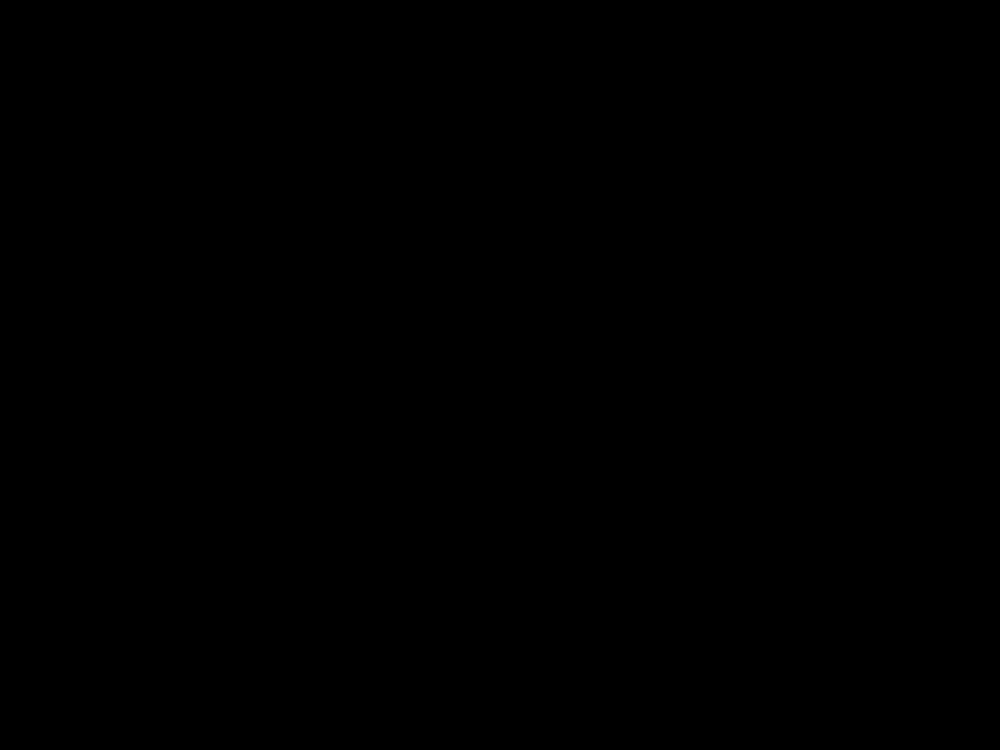
\includegraphics[width=40mm]{images/placeholder.png}}
  \caption{The closed system of 2 colliding particles}
\end{figure}

\begin{gather}
  \int \Sigma F\,dt = \Delta mv\\
  \int (F_A + F_i + F_B - F_i)\,dt = (m_A+m_B)v_2 - (m_A+m_B)v_1\\
  \text{if $F_A = F_B = 0$:} \quad \int F\,dt = 0
\end{gather}

\begin{figure}[h]
  \centering
  \subfloat[Situations]{{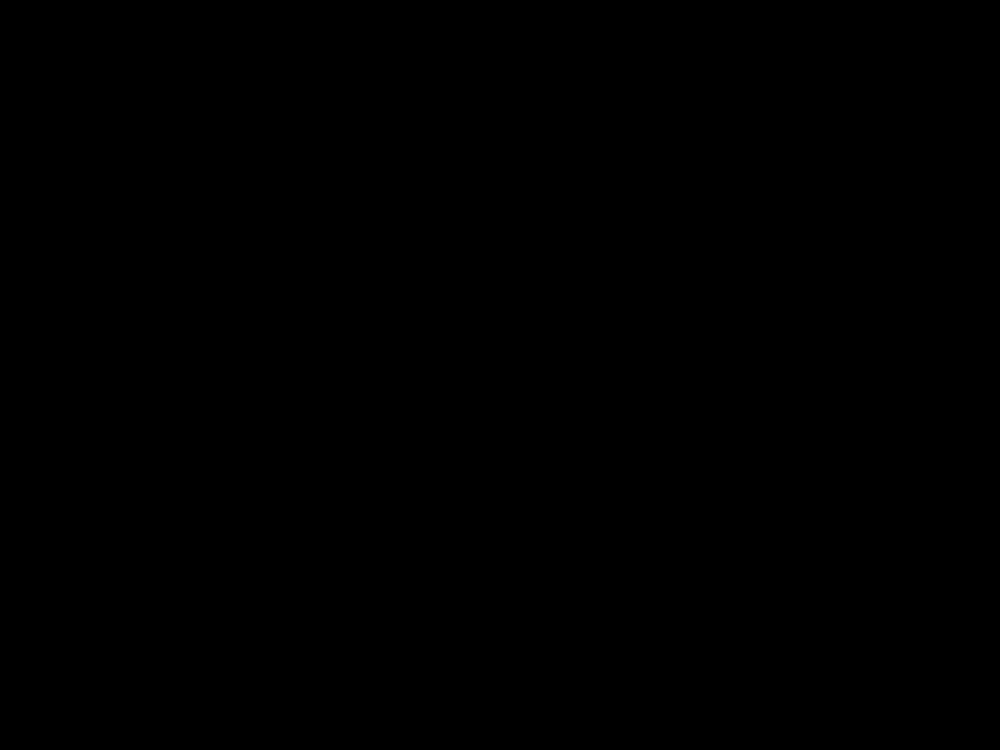
\includegraphics[width=50mm]{images/placeholder.png}}}%
  \qquad
  \subfloat[Graph]{{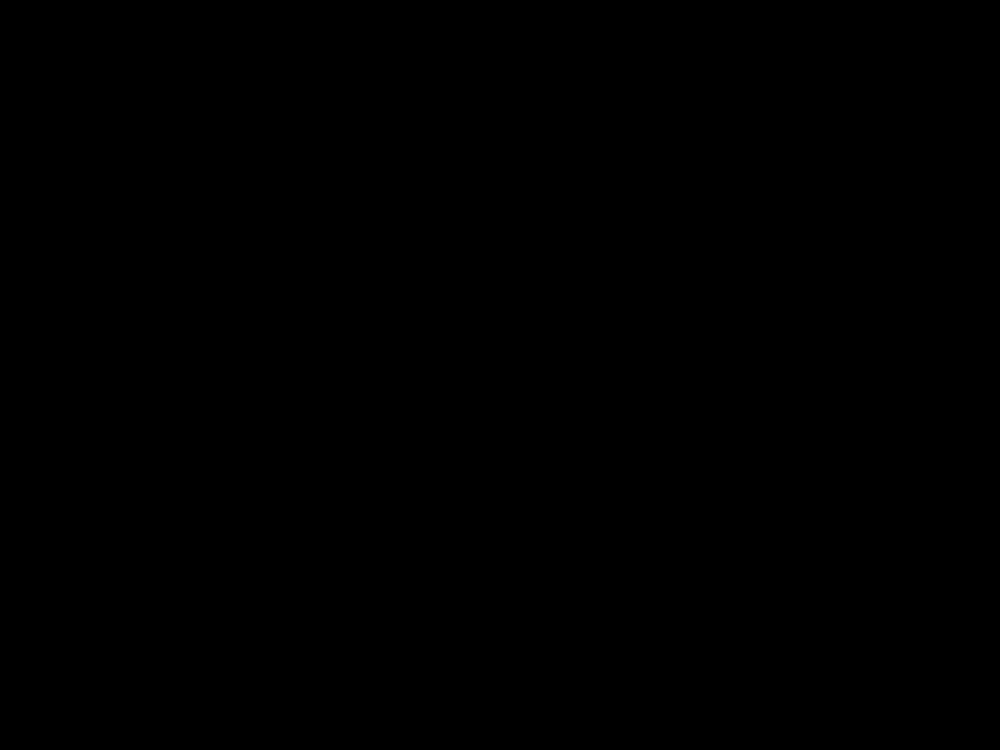
\includegraphics[width=50mm]{images/placeholder.png}}}%
  \caption{The internal force $F_i$ over a time $\Delta t$. Note that $F_i >> F_{ext}$}
\end{figure}
Looking at figure 2 (b) would imply that the internal forces in the system are greater then $0$. However
when we draw the same graph representing impulse for particle B we will find that the impulse is the same but mirrored across the $x$ axes.
This means that the total sum of $F_i$ is still $0$.


\subsection{Coefficient of restitution}
The coefficient of restitution, usually denoted by $e$ is the ratio of final vs initial velocity.
The factor is usually found through experimental data and comparable situations. 
\begin{gather}
  e = \frac{|v_{B2}-v_{A2}|}{|v_{A1}-v_{B1}|}\\
  0 \leq e \leq 1 \notag
\end{gather}
Subsituting in the equation for kinetic energy $E_{kin} = \frac{1}{2}mv^2$ gives the following relation:
\begin{gather}
  e = \sqrt{\frac{E_{kin,2}}{E_{kin,1}}}
\end{gather}
When $e = 0$ the collision is perfectly inelastic. When $e=1$ the collision is perfectly elastic.
The value can possibly be higher then $1$. This would imply that energy was introduced to the system
via some external method, such as a chemical reaction or a reduction in rotational energy.


\subsection{Angled Collisions}
When collision is at an angle the situation should be rotated untill the velocity components can be found 
along and perpendicular tot the impact direction (remember $n,t$-coordinates?).
An example of this can be found in figure 3 (a) and (b) below.
\begin{figure}[h]
  \centering
  \subfloat[Normal]{{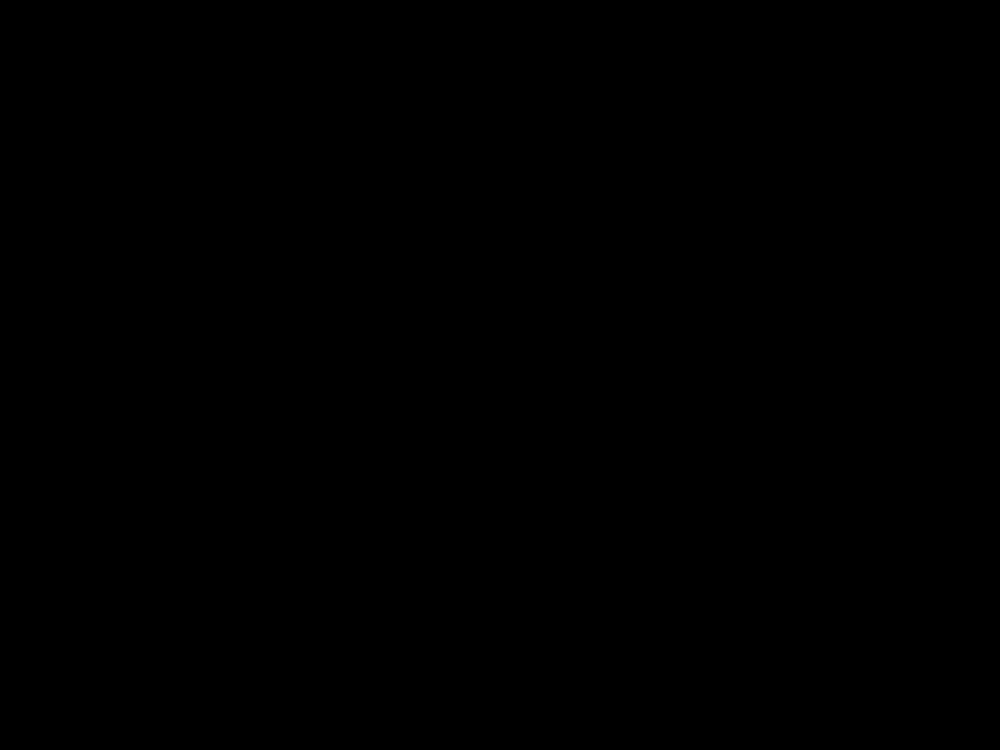
\includegraphics[width=50mm]{images/placeholder.png}}}%
  \qquad
  \subfloat[Rotated]{{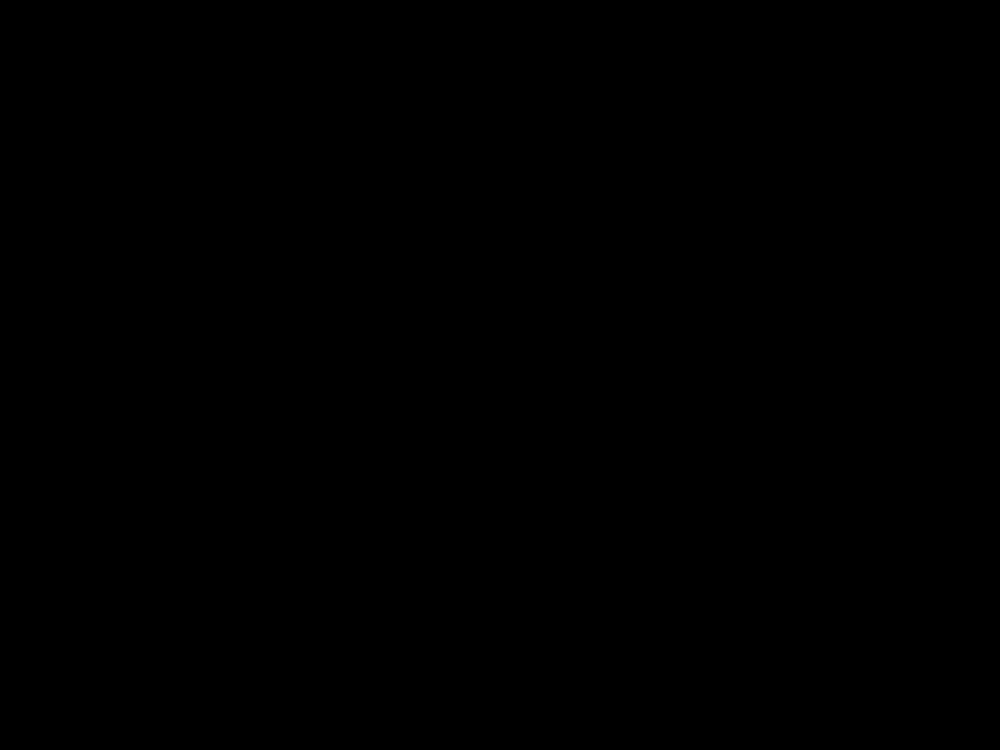
\includegraphics[width=50mm]{images/placeholder.png}}}%
  \caption{Solving a collision problem through rotation untill the tangential and normal components appear.}
\end{figure}



\end{document}